\documentclass{beamer}
\usepackage{beamerthemesplit}
\usepackage{wrapfig}
\usetheme{SPbGU}
\usepackage{pdfpages}
\usepackage{amsmath}
\usepackage{cmap} 
\usepackage[T2A]{fontenc} 
\usepackage[utf8]{inputenc}
\usepackage[english,russian]{babel}
\usepackage{indentfirst}
\usepackage{amsmath}
\usepackage{tikz}
\usepackage{multirow}
\usepackage{subcaption}
\usepackage[noend]{algpseudocode}
\usepackage{algorithm}
\usepackage{algorithmicx}
\usetikzlibrary{shapes,arrows}
\usepackage{fancyvrb}
\newtheorem{rutheorem}{Теорема}
\newtheorem{task}{Задача поиска путей и задача достижимости с контекстно-свободными ограничениями}
\newtheorem{ruproof}{Доказательство}
\newtheorem{rudefinition}{Определение}
\newtheorem{rulemma}{Лемма}
\beamertemplatenavigationsymbolsempty

\title[]{Улучшение производительности алгоритма поиска путей с контекстно-свободными ограничениями для графовой базы данных Neo4j}
% То, что в квадратных скобках, отображается в левом нижнем углу. 
\institute[СПбГУ]{
Санкт-Петербургский государственный университет \\
Кафедра системного программирования }

% То, что в квадратных скобках, отображается в левом нижнем углу.
\author[Погожельская Влада]{Погожельская Влада Владимировна, 18.Б11-мм \\
  % У научного руководителя должна быть указана научная степень
  \and  
    {\bfseries Научный руководитель:} к.\,ф.-м.\,н., доцент кафедры информатики Григорьев С.\,В. \\ 
  % Для курсовой не обязателен. Должна быть указана должность или ученая степень
}
\date{11 июня 2021г.}

\definecolor{orange}{RGB}{179,36,31}

\begin{document}
{
% Лого университета или организации, отображается в шапке титульного листа
\begin{frame}
  \begin{center}
  {\includegraphics[width=1.2cm]{pictures/SPbGU_Logo.png}}
  \end{center}
  \titlepage
\end{frame}
}

\begin{frame}[fragile]
  \transwipe[direction=90]
  \frametitle{Введение}
  \begin{itemize}
      \item Графовая модель представления данных
      \begin{itemize}
        \item Основные сущности --- вершины графа
        \item Взаимосвязи между сущностями хранятся в самой графовой модели
      \end{itemize}
    \item Графовые базы данных
\begin{itemize}
    \item Одной из наиболее распространенных является Neo4j
    \item Для запросов поддерживаются только частично регулярные грамматики
\end{itemize} 
\item Контекстно-свободные ограничения
\begin{itemize}
    \item Строго расширяют выразительность запросов по сравнению с регулярными ограничениями
    \item Имеют широкое применение в биоинформатике, анализе RDF-файлов
\end{itemize}
\end{itemize}
\end{frame}

\begin{frame}[fragile]
  \transwipe[direction=90]
  \frametitle{Задача поиска путей с контекстно-свободными ограничениями}
   \begin{task}
  Дано:
     \begin{itemize}
    \item Контекстно-свободная грамматика $\mathbb{G}  = \langle N, \Sigma, P, S \rangle$
     \item Ориентированный граф $ \mathbb{D} = \langle V, E, T \rangle$
     \item Множество стартовых вершин $V_S \subseteq V$  и финальных вершин \mbox{$V_F \subseteq V$}
\end{itemize} 
\textbf{Задача поиска путей}:
\begin{itemize}
    \item Найти все такие пути $\pi = (e_0, e_1, \cdots, e_{n - 1}, e_n), ~ e_k = (v_{k - 1}, t_k, v_k)$ в графе $ \mathbb{D}$, что $l(\pi) = t_1t_2 \cdots t_n \in L(\mathbb{G})$ и $v_0 \in V_S, ~v_n \in V_F$
\end{itemize}
\textbf{Задача достижимости}:
\begin{itemize}
    \item Найти множество пар $\{(v_i, v_j ) ~|~ \exists ~l(\pi) \in L(\mathbb{G})$ и $v_0 \in V_S, ~v_n \in V_F\}$
\end{itemize}
 \end{task}
\end{frame}

\begin{frame}[fragile]
  \transwipe[direction=90]
  \frametitle{Применение Generalized LL для запросов с контекстно-свободными ограничениями}
  \begin{itemize}
      \item Классический алгоритм синтаксического анализа Generlized LL был обобщен для выполнения контекстно-свободных запросов на графах\footnote{Дипломная работа Власовой А.С.: \url{https://se.math.spbu.ru/thesis/texts/Vlasova_Anna_Sergeevna_Bachelor_Thesis_2020_text.pdf}}
      \item На реальных данных алгоритм в большинстве случаев дал существенный прирост в производительности
      \item При проведении экспериментального исследования выявлено неожиданное ухудшение в поведении полученного решения
      \item На практике восстановление самих путей в графе не всегда требуется
\end{itemize}
\end{frame}

\begin{frame}
  \transwipe[direction=90]
  \frametitle{Цели и задачи}
  \textbf{Целью} данной работы является улучшение производительности алгоритма поиска путей с контекстно-свободными ограничениями для графовой базы данных Neo4j
  
  \textbf{Задачи}:
  \begin{itemize}
    \item Провести анализ и рефакторинг кода с целью выявления и устранения проблем производительности текущей реализации GLL алгоритма
    \item Добавить возможность отключения построения путей и возврата информации лишь о достижимости в графе
    \item Провести экспериментальное исследование на реальных данных и сравнить полученное решение с уже существующим
\end{itemize}
\end{frame}

\begin{frame}
  \transwipe[direction=90]
  \frametitle{Обзор существующего решения}
  \textbf{Обобщенный LL-алгоритм (GLL)}
\begin{itemize}
    \item Поддерживает весь класс контекстно-свободных языков
    \item Для восстановления путей поддерживается сжатое представление леса разбора (SPPF)
\end{itemize}
\textbf{Реализация}\\
  \begin{itemize}
    \item Решение базируется на реализации GLL в библиотеке Iguana\footnote{ Репозиторий библиотеки Iguana: \url{https://github.com/iguana-parser/iguana}}, написанной на Java
    \item В качестве хранилища графов использована графовая база данных Neo4j
    \item Полученное решение интегрировано с Neo4j при помощи Native Java API
  \end{itemize}
  \end{frame}

\begin{frame}
  \transwipe[direction=90]
  \frametitle{Экспериментальное исследование существующего решения}
  Графы:
  \begin{itemize}
    \item Enzyme --- граф о белковых последовательностях (48 тыс. вершин и 86 тыс. ребер)
    \item Geospecies --- граф о таксономической иерархии видов животных (450 тыс. вершин и 2.2 млн ребер)
\end{itemize}
Грамматики:
\begin{align}
\begin{split}
\label{eqn:g_1}
S \to & \overline{\textit{subClassOf}} \ \ S \ \textit{subClassOf} \mid \overline{\textit{type}} \ \ S \ \textit{type}\\   & \mid \overline{\textit{subClassOf}} \ \ \textit{subClassOf} \mid \overline{\textit{type}} \ \textit{type}
\end{split}
\end{align}
\begin{align}
\label{eqn:g_2}
S \to \overline{\textit{subClassOf}} \ \ S \ \textit{subClassOf} \mid \textit{subClassOf}
\end{align}
\begin{align}
\begin{split}
\label{eqn:geo}
S \to & \textit{broaderTransitive} \ \  S \ \overline{\textit{broaderTransitive}} \\
      & \mid \textit{broaderTransitive} \ \  \overline{\textit{broaderTransitive}}
\end{split}
\end{align}
\end{frame}

\begin{frame}
\transwipe[direction=90]
 \frametitle{Экспериментальное исследование существующего решения}
    \begin{figure}[H]
    \begin{subfigure}[b]{0.5\textwidth}
    \centering
    \includegraphics[width=\textwidth]{pictures/subclass_old.pdf_1.jpg} \caption{время выполнения \\ запросов}
    \label{3}
    \end{subfigure}%
    % \hfill
    \begin{subfigure}[b]{0.5\textwidth}
    \centering
    \includegraphics[width=\columnwidth]{pictures/subclass_old_mean&median.pdf_1.jpg} \caption{медиана и среднее время выполнения запросов}
    \label{4}
    \end{subfigure} \caption{Грамматика $G_2$ на Enzyme}
    \label{old2}
    \end{figure}
\end{frame}

\begin{frame}
\transwipe[direction=90]
 \frametitle{Устранение проблем с производительностью}
\begin{itemize}
    \item Наибольшее количество процессорного времени тратилось на сопоставление текущего входа с терминалом грамматики и получение меток на ребрах
    \item Результат обращения к базе данных в явном виде сохранялся в список
    \item Практически всё процессорное время тратилось на вычисления внутри базы данных
\end{itemize}
Предложенное решение:
 \begin{itemize}
     \item После сопоставления входа с терминалом, возможно, далеко не все метки понадобятся для дальнейшей работы алгоритма
     \item Native Java API предоставляет способ получить итератор над множеством исходящих из вершины ребер, а Stream API позволил обеспечить потоковую обработку данных, извлекаемых посредством обращения к Neo4j
 \end{itemize}
\end{frame}

\begin{frame}
\transwipe[direction=90]
 \frametitle{Экспериментальное исследование предложенной реализации}
     \begin{figure}[H]
    \begin{subfigure}[b]{0.5\textwidth}
    \centering
    \includegraphics[width=\textwidth]{pictures/subclass_old_new.pdf_1.jpg} \caption{время выполнения \\ запросов}
    \label{fig:subim1}
    \end{subfigure}%
    % \hfill
    \begin{subfigure}[b]{0.5\textwidth}
    \centering
    \includegraphics[width=\columnwidth]{pictures/subclass_old_new_mean&median.pdf_1.jpg} \caption{медиана и среднее время выполнения запросов}
    \label{fig:subim2}
    \end{subfigure} \caption{Грамматика $G_2$ на Enzyme}
    \label{old_new2}
    \end{figure}
\end{frame}

\begin{frame}
\transwipe[direction=90]
 \frametitle{Модификация алгоритма GLL}
 \begin{figure}[H]
\centering
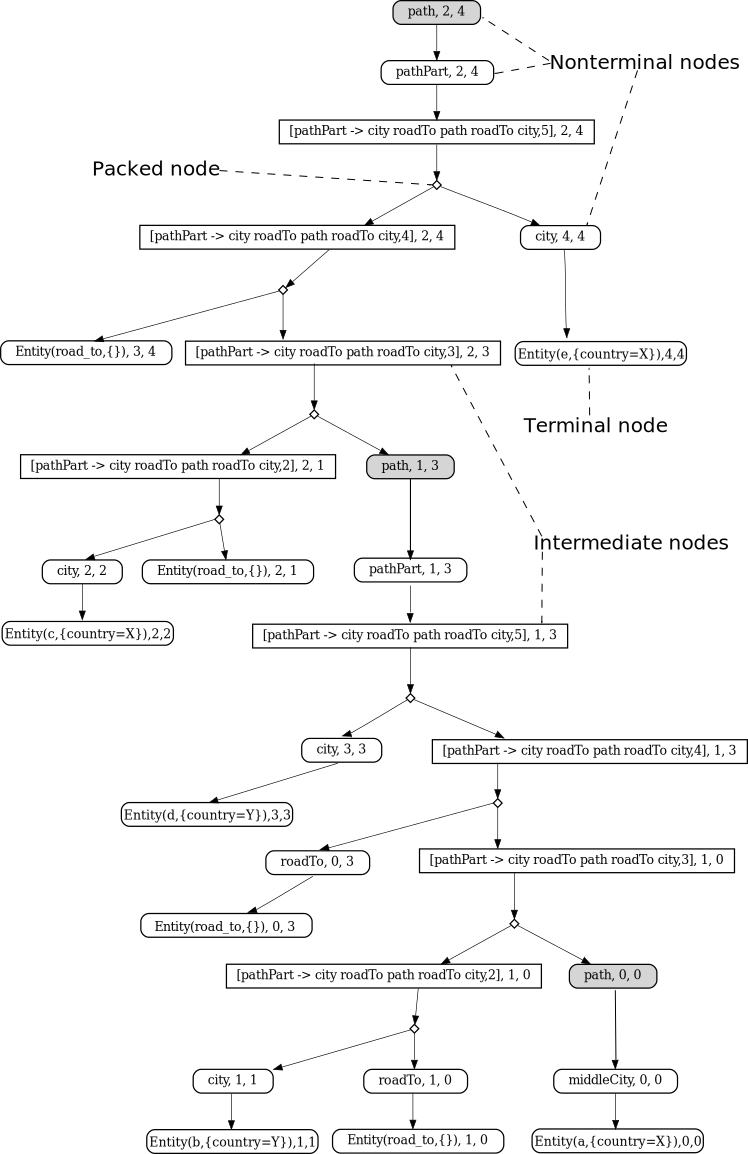
\includegraphics[width=0.9\textwidth]{SlidesTemplate/pictures/sppf.pdf}
\caption{Диаграмма классов Iguana после модификаций для поддержки опции отключения SPPF}
\label{fig:sppf}
\end{figure}
\end{frame}

\begin{frame}
\transwipe[direction=90]
 \frametitle{Экспериментальное исследование модифицированного алгоритма}
          \begin{figure}[H]
    \begin{subfigure}[b]{0.5\textwidth}
    \centering
    \includegraphics[width=\textwidth]{pictures/enzyme_sppf_subclass.pdf_1.jpg} \caption{время выполнения \\ запросов}
    \label{fig:subim1}
    \end{subfigure}%
    % \hfill
    \begin{subfigure}[b]{0.5\textwidth}
    \centering
    \includegraphics[width=\columnwidth]{pictures/enzyme_subclass_ans_st.pdf_1.jpg} \caption{размер ответов \\ на запросы}
    \label{fig:subim2}
    \end{subfigure} \caption{Грамматика $G_2$ на Enzyme}
    \label{old_new2}
    \end{figure}
\end{frame}

\begin{frame}
\transwipe[direction=90]
 \frametitle{Экспериментальное исследование модифицированного алгоритма}
          \begin{figure}[H]
    \begin{subfigure}[b]{0.5\textwidth}
    \centering
    \includegraphics[width=\textwidth]{pictures/geospecies_sppf_bt.pdf_1.jpg} \caption{время выполнения запросов}
    \label{fig:subim3}
    \end{subfigure}%
    % \hfill
    \begin{subfigure}[b]{0.5\textwidth}
    \centering
    \includegraphics[width=\textwidth]{pictures/geospecies_ans_bt.pdf_1.jpg} \caption{размер ответов на запросы}
    \label{fig:subim4} 
    \end{subfigure} \caption{Грамматика $G_3$ на Geospecies}
\label{ssss}
\end{figure}
\end{frame}

\begin{frame}
\transwipe[direction=90]
 \frametitle{Выводы}
\begin{itemize}
    \item Модифицированный алгоритм GLL без построения SPPF может быть эффективно применен для решения задачи достижимости в графе с контекстно-свободными ограничениями на реальных данных
    \item Полученные результаты делают актуальными дальнейшие исследования, направленные как на улучшение данного алгоритма и реализации, так и на полноценную интеграцию его в графовую базу данных Neo4j
\end{itemize}
\end{frame}

\begin{frame}
\transwipe[direction=90]
 \frametitle{Заключение}
В рамках производственной практики были выполнены следующие задачи
\begin{itemize}
    \item Проведен анализ и рефакторинг кода
    \item Выявлены и устранены проблем производительности текущей реализации GLL алгоритма
    \item Добавлена возможность отключения построения SPPF и возврата информации лишь о достижимости в графе
    \item Проведено экспериментальное исследование на реальных данных и сравнение полученного решения с уже существующим
\end{itemize}
\end{frame}
\end{document}